\documentclass[10pt,a4paper]{article}
\usepackage[utf8]{inputenc}
\usepackage{amsmath}
\usepackage{amsfonts}
\usepackage{amssymb}
\usepackage{amsthm}
\usepackage{mathtools}
\usepackage{geometry}[margin=1in]
\usepackage{tikz}
\usetikzlibrary{arrows}
\usepackage[parfill]{parskip}
\usepackage{subcaption}
\usepackage{stmaryrd}
\newcommand{\st}{\text{ s.t. }}
\newcommand{\contr}{\lightning}
\newcommand{\im}{\mathfrak{i}}
\newcommand{\R}{\mathbb{R}}
\newcommand{\Q}{\mathbb{Q}}
\newcommand{\C}{\mathbb{C}}
\newcommand{\F}{\mathbb{F}}
\newcommand{\K}{\mathbb{K}}
\newcommand{\N}{\mathbb{N}}
\newcommand{\Z}{\mathbb{Z}}
\DeclareMathOperator{\id}{id}
\let\emph\relax
\DeclareTextFontCommand{\emph}{\bfseries\em}
\setcounter{section}{-1}

\newtheorem{ctsDiscToSphere}{Theorem}[section]
\newtheorem{lem11}{Lemma}[section]
\newtheorem{lem12}[lem11]{Lemma}
\newtheorem{thm13}[lem11]{Theorem}
\newtheorem{lem14}[lem11]{Lemma}
\newtheorem{lem15}[lem11]{Lemma}
\newtheorem{lem16}[lem11]{Lemma}
\newtheorem{lem17}[lem11]{Lemma}

\title{Algebraic Topology}
\begin{document}
\maketitle

\section{Introduction}
The fundamental problem of topology is to establish whether or not there exist continuous functions $f, g$ going from a topological space $X$ to another space $Y$ and back again. For example, in the case of this torus and double-torus, we know from Geometry that such functions cannot exist by considering the Euler characteristic, but in general this is a hard problem.
\begin{center}
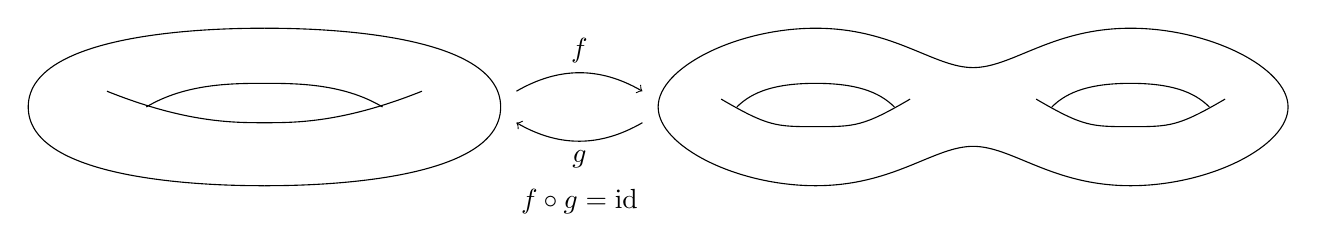
\begin{tikzpicture}
\draw (-7,0) .. controls (-7,1) and (-4.4,1) .. (-4,1);
\draw (-7,0) .. controls (-7,-1) and (-4.4,-1) .. (-4,-1);
\draw (-1,0) .. controls (-1,1) and (-3.6,1) .. (-4,1);
\draw (-1,0) .. controls (-1,-1) and (-3.6,-1) .. (-4,-1);
\draw (-5.5,0) .. controls (-5,0.3) and (-4.4,0.3) .. (-4,0.3) .. controls (-3.6,0.3) and (-3,0.3) .. (-2.5,0);
\draw (-6,0.2) .. controls (-5,-0.2) and (-4.4,-0.2) .. (-4,-0.2) .. controls (-3.6,-0.2) and (-3,-0.2) .. (-2,0.2);

\draw (1,0) .. controls (1,0.5) and (2,1) .. (3,1) .. controls (4,1) and (4.5,0.5) .. (5,0.5) .. controls (5.5,0.5) and (6,1) .. (7,1) .. controls (8,1) and (9,0.5) .. (9,0);
\draw (1,0) .. controls (1,-0.5) and (2,-1) .. (3,-1) .. controls (4,-1) and (4.5,-0.5) .. (5,-0.5) .. controls (5.5,-0.5) and (6,-1) .. (7,-1) .. controls (8,-1) and (9,-0.5) .. (9,0);
\draw (2,0) .. controls (2.2,0.2) and (2.5,0.3) .. (3,0.3) .. controls (3.5,0.3) and (3.8,0.2) .. (4,0);
\draw (1.8,0.1) .. controls (2.4,-0.25) and (2.5,-0.25) .. (3,-0.25) .. controls (3.5,-0.25) and (3.6, -0.25) .. (4.2,0.1);
\draw (6,0) .. controls (6.2,0.2) and (6.5,0.3) .. (7,0.3) .. controls (7.5,0.3) and (7.8,0.2) .. (8,0);
\draw (5.8,0.1) .. controls (6.4,-0.25) and (6.5,-0.25) .. (7,-0.25) .. controls (7.5,-0.25) and (7.6, -0.25) .. (8.2,0.1);

\draw (-0.8,0.2) edge[bend left, ->] node[above] {$f$} (0.8,0.2);
\draw (0.8,-0.2) edge[bend left, ->] node[below] {$g$} (-0.8,-0.2);
\node at (0,-1.2) {$f \circ g = \id$};
\end{tikzpicture}
\end{center}
If such $f, g$ continuous functions exist, then we say the two spaces are homeomorphic. Basic idea of algebraic topology is that we want to associate to any topological space $X$ a group $G(X)$, and for every continuous function $f:X \rightarrow Y$ a group homomorphism $G(f): G(X) \rightarrow G(Y)$ with $G(\id) = \id$ and $G(f\circ g)=G(f)\circ G(g)$. Thus if $f:X\rightarrow Y$ is a homeomorphism with inverse $g:Y\rightarrow X$, then $G(g)\circ G(f)=\id, G(f)\circ G(g) = \id$, so $G(f)$ is an is an isomorphism.

\underline{Extension problem:} Let $X$ be a topological space, $A\subseteq X$ a subspace, and $f:A\rightarrow Y$ a continuous function. Does there exist a continuous function $F:X\rightarrow Y$ with $F|_A = f$
\begin{center}
\tikz{
\node (A) at (0,0) [circle] {$A$};
\node (X) at (0,2) [circle] {$X$};
\node (Y) at (2,2) [circle] {$Y$};
\draw (A) edge[right hook->] (X);
\draw (X) edge[dashed,->] node[below] {$\exists$?}(Y);
\draw (A) edge[->] node[below] {$f$} (Y);
}
\end{center}
\begin{ctsDiscToSphere}
There is no continuous function
\begin{center} $f:D^n \rightarrow S^{n-1}$ with $f|_{S^{n-1}} = \id$\end{center}
\end{ctsDiscToSphere}
By hand, we can see why this fails for e.g. $n=1, 2$, but it gets hard to generalise. Eventually, we will construct $G$ with $G(D^n) = 0, G(S^{n-1}) = \Z$. Then, if we have $S^{n-1} \rightarrow D^n \rightarrow S^{n-1}$ with composition being the identity, then we have maps $\Z \rightarrow 0 \rightarrow \Z$ being the identity.

\subsection*{Conventions}
A topological space will be referred to as a \emph{space}\\
A continuous function $f:X\rightarrow Y$ will be called a \emph{map}

\section{The Fundamental Group}
The idea here is that, if $X$ is a space, $x_0 \in X$ a fixed point, called the \emph{basepoint}, we consider loops based at $x_0$, i.e. maps $\gamma:[0,1] \rightarrow X$ with $\gamma(0) = \gamma(1) = x_0$.

For example, if we let our space $X = \R^2\setminus \{0\}$

\begin{figure}
\begin{center}
\tikz{
\draw (0,0) rectangle ++(5,5);
\node[fill, draw, circle, minimum width=3pt, inner sep=0pt, label={270:$x_0$}] (x) at (2,1.5) {};
\node[fill, draw, circle, minimum width=3pt, inner sep=0pt, label={0:$0$}] (o) at (2.5,2.5) {};
\draw[green!80!black] plot [smooth cycle, tension=1.2] coordinates {(x) (4,2.5) (3,3) (2,2.5)};
\draw[red!90!black] plot [smooth cycle, tension=1.2] coordinates {(x) (4,1.5) (4.5,3) (2.5,4) (1,2.5)};
\draw[blue] plot [smooth cycle] coordinates {(x) (0.5,0.5) (2.5,0.5) (2,1) (1,0.5)};
}
\end{center}
\caption*{Here, the green and red loops are the ``same" loop, whilst the blue one is distinct}
\end{figure}

Then the \emph{fundamental group} $\pi_1(X) = \pi_1(X, x_0)$ is defined to be the set of loops based at $x_0$ modulo ``deforming loops". Multiplication in this group $\gamma_1 \cdot \gamma_2$ is given by first traversing $\gamma_1$ and then $\gamma_2$. But what do we mean by ``deforming" a loop?

Let $f_0, f_1: X \rightarrow Y$ be maps. A \emph{homotopy} between $f_0$ and $f_1$ is a map
\begin{align*}
F:X\times I &\rightarrow Y \text{ where $I=[0,1]$ and}\\
F(x,0) &= f_0(x) \text{ and }\\
F(x,1) &= f_1(x)
\end{align*}
We often write $f_\tau(x) = F(x,\tau), f_\tau:X\rightarrow Y$.

If such $F$ exists, we say $f_0$ and $f_1$ are \emph{homotopic}.

\underline{Example:} Let $Y\subseteq \R^2$ be a convex set. Then any $f_0, f_1:X\rightarrow Y$ are homotopic, via $F(x,t) = tf_1(x) + (1-t)f_0(x) \in Y$ by convexity.
\begin{center}
\tikz{
\draw (0,0) circle[radius=2cm];
\node[fill, draw, circle, minimum width=3pt, inner sep=0pt, label={270:$f_1(x)$}] (a) at (-1,0.6) {};
\node[fill, draw, circle, minimum width=3pt, inner sep=0pt, label={330:$f_2(x)$}] (b) at (0.5,1.5) {};
\draw (a) edge node[fill, draw, circle, minimum width=3pt, inner sep=0pt, label={300:$f_\tau(x)$}] {} (b);
}
\end{center}

If $f_0$ is homotopic to $f_1$, we write $f_0 \simeq f_1$, or $f_0 \simeq_F f_1$ if we want to be explicit about the homotopy we are using.

Suppose $f_0 \simeq_F f_1$, both functions $X \rightarrow Y$. If $Z\subseteq X$ and $f_0(z)=F(z,t) = f_1(z) \forall z \in Z, t \in I$, then we say $f_0$ is homotopic to $f_1$ \emph{relative to} $Z$.

\begin{lem11}
Let $Z\subseteq X, Y$ be spaces. Then $\simeq$ relative to $Z$ is an equivalence relation on the set of maps $X\rightarrow Y$.
\end{lem11}
\begin{proof}
\item
\begin{itemize}
\item{Reflexive: } $f_0 \simeq f_0$ via $F(x,t) = f_0(x) \forall x,t$
\item{Symmetric: } Given $f_0\simeq_F f_1$, then $f_1 \simeq f_0$ via $F'(x,t) = f(x, 1-t)$
\item{Transitive: } If $f_0 \simeq_{F_0} f_1, f1 \simeq_{F_1} f_2$, then $f_0 \simeq_F f_2$ with:
\begin{align*}
F(x,t) =
\begin{cases} 
F_0(x,2t) & t\leq 1/2 \\
F_1(x,2t-1) & t \geq 1/2
\end{cases}
\end{align*}
All homotopies are relative to $Z$.
\end{itemize}
\end{proof}
A \emph{homotopy equivalence} $f:X\rightarrow Y$ is a map with a \emph{homotopy inverse} $g:Y\rightarrow X$ such that $f\circ g = \id_Y, g\circ f = \id_X$. We then write $X \simeq Y$.

\underline{Remark:} Most (all?) invariants in the course are \emph{homotopy invariants}

Examples:
\begin{enumerate}
\item Let $\ast$ be the one point space, $f:\R^n \rightarrow \ast$ be the constant map, and let $g:\ast \rightarrow \R^n; x\mapsto \mathbf{0}$. Then $f\circ g = \id_{\ast}$, and $g\circ f (x) = 0 \forall x\in\R^n$. Now $g\circ f \simeq \id_{\R^n}$ via $F(x,t) = tx$.
\item Let $f:S^{n-1} \hookrightarrow \R^n\setminus\{0\}$ be the inclusion map, and $g:\R^n\setminus\{0\} \rightarrow S^{n-1}; x\mapsto \frac{x}{|x|}$ (i.e. map $x$ to the intersection of $\overrightarrow{\mathbf{0}x}$ with $S^{n-1}$) . Then $g\circ f =\id_{S^{n-1}}$ and $f\circ g \simeq \id_{\R^n\setminus\{0\}}$ via $F(x,t) = (1-t)x + t\cdot\frac{x}{|x|}$
\end{enumerate}

If $X\simeq \ast$, then we say $X$ is \emph{contractible}.\\
Let $f:X\rightarrow Y, g:Y\rightarrow X$ be maps. If $g\circ f=\id_X$, then we say $X$ is a \emph{retract} of $Y$, and $g$ is a \emph{retraction}. If in addition $f\circ g\simeq \id_Y$ relative to $f(X)$, then we say $X$ is a \emph{deformation retract} of $Y$. Hence, in example 2, we see that $S^{n-1}$ is a deformation retract of $\R^n$.

\begin{lem12}
Homotopy equivalence of spaces is an equivalence relation.
\end{lem12}
\begin{proof}
Reflexivity and symmetry are trivial from the definition.

Suppose $X\simeq Y, Y\simeq Z$ via:
\begin{center}
\tikz{
\node (x) at (0,0) {$X$};
\node (y1) at (2,0) {$Y$};
\node (y2) at (4,0) {$Y$};
\node (z) at (6,0) {$Z$};
\draw (x) edge[bend left, ->] node[above] {$f$} (y1);
\draw (y1) edge[bend left, ->] node[below] {$g$} (x);
\draw (y2) edge[bend left, ->] node[above] {$f'$} (z);
\draw (z) edge[bend left, ->] node[below] {$g'$} (y2);
}
\end{center}
We want to show $f'\circ f$, $g\circ g'$ induces a homotopy equivalence
\begin{center}
\tikz{
\node (x) at (0,0) {$X$};
\node (z) at (2,0) {$Z$};
\draw (x) edge[bend left, ->] node[above] {$f'\circ f$} (z);
\draw (z) edge[bend left, ->] node[below] {$g\circ g'$} (x);
}
\end{center}

Now $(g\circ g') \circ(f'\circ f) = g\circ (g'\circ f')\circ f$. We know already that $g'\circ f' \simeq_{F'} \id_Y$, and so:
\begin{align*}
(x,t) \mapsto g(F'(f(x), t)) = \begin{cases} g(g'(f'(f(x)))) & t=0 \\ g(f(x)) & t =1 \end{cases}
\end{align*}
is a  homotopy, as $g\circ (g'\circ f')\circ f \simeq g\circ f$, and since $X\simeq Y$, $g\circ f \simeq \id_X$. Hence $(g\circ g')\circ (f'\circ f) \simeq \id_X$ via transitivity of homotopy equivalence for maps. Similarly $(f'\circ f)\circ (g\circ g') \simeq \id_Z$
\end{proof}

\subsection*{Loops and $\mathbf{\pi_1}$}
If $X$ is a space, a \emph{path} in $X$ is a map $\gamma:I \rightarrow X$, where $I = [0,1]\subseteq \R$. If $\gamma(0) = x_0, \gamma(1) = x_1$ then we say $\gamma$ is a path \emph{from $x_0$ to $x_1$}.\\
We say $\gamma_1$ and $\gamma_2$ are \emph{homotopic} if $\gamma_1\simeq \gamma_2$ relative to $\{0, 1\}$, and we write $[\gamma]$ for the homotopy equivalence class of $\gamma$.

If $X$ is a space with points $x,y,z \in X$, and $\gamma_1$ is a path from $x$ to $y$, $\gamma_2$ is a path from $y$ to $z$, then:
\begin{itemize}
\item The \emph{concatenation} of $\gamma_1$ and $\gamma_2$ is the path from $x$ to $z$ given by
\begin{align*}
(\gamma_1 \cdot \gamma_2) (s) = \begin{cases} \gamma_1(2s) & 0\leq s\leq 1/2 \\ \gamma_2(2s-1) & 1/2\leq s\leq 1\end{cases}
\end{align*}
\item The \emph{constant path} at $x$ is the path $c_x(s) = x \forall s \in I$
\item The \emph{inverse of} $\gamma_1$ is $\overline{\gamma_1}(s) = \gamma_1(1-s)$, a path from $y$ to $x$.
\end{itemize}
\begin{center}
\tikz{
\node (x) at (0,0) {$x$};
\node (y) at (2,0) {$y$};
\node (z) at (4,0) {$z$};
\draw (x) edge[bend left, green!60!black, ->] node[below, green!60!black] {$\gamma_1$} (y);
\draw (y) edge[bend right, red!60!black, ->] node[above, red!60!black] {$\gamma_2$} (z);
\draw (x) edge[bend left, blue!60!black, ->] node[above, blue!60!black] {$\gamma_1 \cdot \gamma_2$} (z);
\draw (y) edge[bend left, red!50!blue, ->] node[below] {$\overline{\gamma_1}$} (x);
}
\end{center}

\begin{thm13}
Let $X$ be space, and $x_0 \in X$. Let $\pi_1(X,x_0)$ be the set of homotopy classes of loops in $X$ with endpoint $x_0$ (we say they are \emph{based} at $x_0$). Then $\pi_1(X,x_0)$ forms a group under the product $[\gamma_1][\gamma_2] = [\gamma_1\cdot\gamma_2]$, with identity $c_{x_0}$ and inverses $[\gamma_1]^{-1} = [\overline{\gamma_1}]$.

This group is called the \emph{fundamental group} of $X$ (based at $x_0$).
\end{thm13}

To prove this, we will need the following lemmas:
\begin{lem14}
If $\gamma_0\simeq \gamma_1$ to $y$ and $\delta_0\simeq \delta_1$ from $y$, then $\gamma_0 \cdot \delta_0 \simeq \gamma_1\cdot \delta_1$ and $\overline{\gamma_0} \simeq \overline{\gamma_1}$
\begin{center}
\tikz{
\node (x) at (0,0) {};
\node (y) at (2,0) {$y$};
\node (z) at (4,0) {};
\draw (x) edge[bend left, green!60!black, ->] node[above, green!60!black] {$\gamma_0$} (y);
\draw (x) edge[bend right, green!60!black, ->] node[below, green!60!black] {$\gamma_1$} (y);
\draw (y) edge[bend right, red!60!black, ->] node[below, red!60!black] {$\delta_1$} (z);
\draw (y) edge[bend left, red!60!black, ->] node[above, red!60!black] {$\delta_0$} (z);
}
\end{center}
\end{lem14}
\begin{proof}
Suppose $\gamma_0\simeq_F \gamma_1$, and $\delta_0\simeq_G \delta_1$. Set:
\begin{align*}
H(s,t) = \begin{cases} F(2s, t) & 0\leq s\leq 1/2 \\ G(2s-1,t) & 1/2 \leq s \leq 1\end{cases}
\end{align*}
Then $\gamma_0\cdot\delta_0 \simeq_H \gamma_1\cdot \delta_1$

Let $F'(s,t) = F(1-s,t)$. Then $\overline{\gamma_0} \simeq_{F'} \overline{\gamma_1}$.
\end{proof}

\begin{lem15}
Let $\alpha, \beta, \gamma$ be paths from $w$ to $x$ to $y$ to $z$ in $X$. 
\begin{center}
\tikz{
\node (w) at (0,0) {$w$};
\node (x) at (2,0) {$x$};
\node (y) at (4,0) {$y$};
\node (z) at (6,0) {$z$};
\draw (w) edge[->, red!60!black, bend left] node[below] {$\alpha$} (x);
\draw (x) edge[->, green!70!black, bend right] node[above] {$\beta$} (y);
\draw (y) edge[->, blue!80!black, bend left] node[below] {$\gamma$} (z);
}
\end{center}
Then:
\begin{enumerate}
\item $(\alpha\cdot \beta)\cdot \gamma \simeq \alpha\beta\cdot \gamma$
\item $\alpha\cdot c_x \simeq \alpha \simeq c_w \cdot \alpha$
\item $\alpha \cdot \overline{\alpha} \simeq c_w$
\end{enumerate}
\end{lem15}

\begin{proof}
First, given a path $\delta:I\rightarrow X$, a \emph{reparametrization} of $\delta$ is a path $\delta \circ \phi$ where $\phi:I\rightarrow I$ is a map with $\phi(0) = 0, \phi(1) = 1$. Note that $\phi$ needn't be monotonic, and that $\delta \simeq \delta \circ \phi$ via $F(s,t) = \delta(t\phi(s) + (1-t)s)$, and this homotopy is relative to $\{0,1\}$. 
\begin{enumerate}
\item Now we reparametrize $(\alpha \cdot \beta)\cdot \gamma$ via the function $\phi$ whose plot is:
\begin{center}
\tikz{
\draw[step=1.0,black,thin] (0.5,0.5) grid (5.5,5.5);
\draw[red!60!black, line width=0.5mm] (1,1) -- (3,2) -- (4,3) -- (5,5);
}
\end{center}
Note that $((\alpha\cdot \beta)\cdot \gamma)\circ \phi = \alpha\cdot(\beta\cdot\gamma)$, so $(\alpha\cdot\beta)\cdot\gamma \simeq \alpha\cdot(\beta\cdot\gamma)$.

\item Reparametrize $\alpha$ via:
\begin{center}
\tikz{
\draw[step=1.0,black,thin] (0.5,0.5) grid (5.5,5.5);
\draw[red!60!black, line width=0.5mm] (1,1) -- (3,1) -- (5,5);
}
\end{center}
i.e. do $c_w$ for the first half of the time, then do $\alpha$, so $\alpha\simeq c_w\cdot \alpha$. Likewise, we can get $\alpha\simeq \alpha\cdot c_x$ using the reparametrization
\begin{center}
\tikz{
\draw[step=1.0,black,thin] (0.5,0.5) grid (5.5,5.5);
\draw[red!60!black, line width=0.5mm] (1,1) -- (3,5) -- (5,5);
}
\end{center}
\item use the homotopy:
\begin{align*}
F(s,t) = \begin{cases} \alpha(2s) & 0\leq s\leq t/2 \\ \alpha(t) & t/2\leq s\leq 1-t/2 \\ \alpha(2-2s) & 1-t/2 \leq s \leq 1 \end{cases}
\end{align*}
So $c_w \simeq \alpha \cdot \bar{\alpha}$, as we have $c_w$ at $t=0$ and $\alpha\cdot\bar{\alpha}$ at $t=1$.
\end{enumerate}
\end{proof}
Then theorem \textbf{1.3} giving the existence of $\pi_1(X, x_0)$ follows from the previous two lemmas.

\underline{Example:} $X=\R^n, x_0 = 0$. If $\gamma$ is a loop based at $0$, then $\gamma\simeq c_0$ via the straight line homotopy, and so $\pi_1(\R^n, 0) = 0$.

\subsection*{Formal Properties of $\pi_1$}
\begin{lem16}
Let $f:X\rightarrow Y$ be a map with $f(x_0) = y_0$. Then there is a homomorphism $f_{\ast}:\pi_1(X,x_0)\rightarrow\pi_1(Y,y_0)$ given by $f_\ast([\gamma]) = [f\circ \gamma]$.

Furthermore:
\begin{enumerate}
\item If $f\simeq f'$ relative to $x_0$, then $f_\ast ' = f_\ast$.
\item If $g:Y\rightarrow Z$ with $g(y_0) = z_0$, then $g_\ast \circ f_\ast = (g\circ f)_\ast$
\item $(\id_X)_\ast = \id_{\pi_1(X,x_0)}$
\end{enumerate}
\end{lem16}

\begin{proof}
$f_\ast$ is well-defined: if $\gamma_1 \simeq_F \gamma_2$, then $f\circ\gamma_1 \simeq_{f\circ F} f\circ \gamma_2$. Then $f\circ(\gamma_1\cdot \gamma_2) = (f\circ \gamma_1)\cdot(f\circ \gamma_2)$ by definition, and so we have a group homomorphism.
\begin{enumerate}
\item If $f\simeq_F f'$ relative to $x_0$, then for $\gamma$ a loop based at $x_0$, $(s,t)\mapsto F(\gamma(s),t)$ is a homotopy between $f\circ \gamma$ and $f'\circ \gamma$.
\item and 3. are immediate by definition.
\end{enumerate}
\end{proof}

\begin{lem17}
let $X$ be a space, $x_0, x_1 \in X$ and $\alpha$ a path from $x_0$ to $x_1$. Then there is a group isomorphism $\alpha_\#:\pi_1(X,x_0)\rightarrow\pi_1(X,x_1)$ via $\alpha_\#([\gamma]) = [\bar{\alpha}\cdot\gamma\cdot\alpha]$.
\begin{center}
\tikz{
\draw (0,0) circle (2cm);
\node[fill, draw, circle, minimum width=3pt, inner sep=0pt, label={330:$x_0$}] (x_0) at (-0.6,-0.3) {};
\node[fill, draw, circle, minimum width=3pt, inner sep=0pt, label={330:$x_1$}] (x_1) at (+0.8,+0.7) {};
\draw[bend left, green!60!black, ->] (x_0) -- node[below right] {$\alpha$} (x_1);
\draw[->, red!60!black] (x_0.120) .. controls (-0.8,-0.2) and (-1,-0.4) .. (-1,-0.6) .. node[left=8] {$\gamma$} controls (-0.9,-0.9) and (-0.55,-0.5) .. (x_0.300);
\draw[->, blue!80!black] (x_1) .. controls (0.7,0.8) and (-0.6,-0.25) .. node[above left] {$\alpha_\#([\gamma])$} (x_0) .. controls (-0.8,-0.1) and (-1.1,-0.4) .. (-1.1,-0.6) .. controls (-0.9,-1) and (-0.55,-0.6) .. (x_0.300) .. controls (-0.57,-0.33) and (0.8,0.6) .. (x_1);
}
\end{center}
Furthermore,
\begin{enumerate}
\item If $\alpha\simeq \alpha'$ relative to $\{0,1\}$, then $\alpha_\# = \alpha'_\#$.
\item $(c_{x_0})_\# = \id_{\pi_1(X,x_0)}$
\item If $\beta$ is a path from $x_2$ to $x_2$, then $(\alpha\cdot\beta)_\# = \beta_\#\circ \alpha_\#$
\item If $f:X\rightarrow Y$ and $y_1=f(x_1)$, then $(f\circ\alpha)_\#\circ f_\ast = f_\ast\circ\alpha_\#$.
\end{enumerate}
\end{lem17}

\begin{proof}
Well-defined: If $\gamma_1\simeq_F\gamma_2$ then $\bar{\alpha}\cdot\gamma_1\cdot\alpha\simeq\bar{\alpha}\cdot\gamma_2\cdot\alpha$ via:
\begin{center}
\tikz{
\draw (0,0)--(0,4)-- node[above] {$\overline{\alpha}$} (2,4) -- node[above] {$\gamma_2$} (4,4) -- node[above] {$\alpha$} (6,4) -- (6,0);
\draw (0,0)-- node[below] {$\overline{\alpha}$} (2,0) -- node[below] {$\gamma_1$} (4,0) -- node[below] {$\alpha$} (6,0);
\draw (2,0) -- (2,4); \draw (4,0) -- (4,4);
\node at (1,2) {\begin{tabular}{c} Trivial \\ Homotopy \end{tabular}};
\node at (3,2) {$F$};
\node at (5,2) {\begin{tabular}{c} Trivial \\ Homotopy \end{tabular}};
\draw[->] (-0.5,0) -- node[left] {$t$} (-0.5,2);
\draw[->] (0,-0.7) -- node[below] {$s$} (2,-0.7);
}
\end{center}
This is indeed a group homomorphism: for loops $\gamma, \delta$ based at $x_0$,
\begin{align*}
\bar{\alpha}\cdot\gamma\cdot\alpha)\cdot(\bar{\alpha}\cdot\delta\cdot\alpha) &\simeq (\bar{\alpha}\cdot\gamma)\cdot(\alpha\cdot\bar{\alpha})\cdot(\delta\cdot\alpha)\\
&\simeq (\bar{\alpha}\cdot\gamma)(c_{x_0})(\delta\cdot\alpha)\\
&\simeq (\bar{\alpha}\cdot\gamma)\cdot(\delta\cdot\alpha)\\
&\simeq \bar{\alpha}\cdot(\gamma\cdot\delta)\cdot\alpha
\end{align*}
Thus $\alpha_\#(\gamma\cdot\delta) = \alpha_\#(\gamma)\cdot\alpha_\#(\delta)$. Also $\bar{\alpha_\#} = (\alpha_{\#})^{-1}$ - this is easy to check. Thus $\alpha_\#$ is a group isomorphism.
\begin{enumerate}
\item If $\alpha\simeq_F \alpha'$
\begin{center}
\tikz{
\draw (0,0)--(0,4)-- node[above] {$\overline{\alpha'}$} (2,4) -- node[above] {$\gamma$} (4,4) -- node[above] {$\alpha'$} (6,4) -- (6,0);
\draw (0,0)-- node[below] {$\overline{\alpha}$} (2,0) -- node[below] {$\gamma$} (4,0) -- node[below] {$\alpha$} (6,0);
\draw (2,0) -- (2,4); \draw (4,0) -- (4,4);
\node at (1,2) {$\overline{F}$};
\node at (3,2) {\begin{tabular}{c} Trivial \\ Homotopy \end{tabular}};
\node at (5,2) {$F$};
\draw[->] (-0.5,0) -- node[left] {$t$} (-0.5,2);
\draw[->] (0,-0.7) -- node[below] {$s$} (2,-0.7);
}
\end{center}
gives $\alpha_\#(\gamma)\simeq\alpha_\#'(\gamma)$
\item Immediate since $c_{x_0}$ is the identity in $\pi_1(X,x_0)$.
\item 
\begin{align*}
(\alpha\cdot\beta)_\#(\gamma) &= \bar{\alpha\cdot\beta} \cdot \gamma\cdot\alpha\cdot\beta\\
&=\bar{\beta}\cdot(\bar{\alpha}\cdot\gamma\cdot\alpha\cdot\beta\\
&= \bar{\beta}\cdot\alpha_\#(\gamma)\cdot \beta\\
&= \beta_\#(\alpha_\#(\gamma))
\end{align*}
\item
\begin{align*}
((f\circ\alpha)_\#\cdot f_\ast)(\gamma) &= (f\circ \alpha)_\#(f\cdot \gamma)\\
&= (f\circ\alpha)_\#(f\cdot\gamma)\\
&= \overline{f\cdot\alpha}\cdot(f\circ\gamma)\cdot(f\circ\alpha)\\
&= f\circ(\bar{\alpha}\cdot\gamma\cdot\alpha)\\
&= f_\ast(\alpha_\#(\gamma))
\end{align*}
\end{enumerate}
\end{proof}



\end{document}
